% !TEX root = ../../../main.tex
% 来源：中学数学实验教材·第三册（高中数学）
% 章节：三角函数的图象和性质 / 余弦函数的图象和性质
% 原始文件：7.tex，行 650-674
% 类型：tikz
% ---
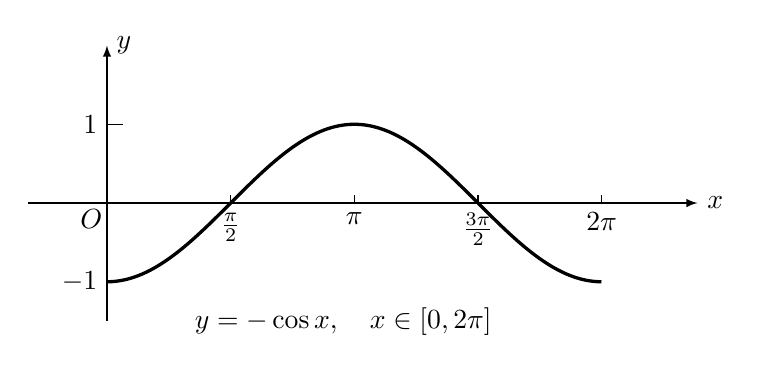
\begin{tikzpicture}[>=latex, xscale=1]
\draw[->](-1,0)--(7.5,0)node[right]{$x$}; 
\draw [->](0,-1.5)--(0,2)node[right]{$y$};
    
\draw[domain=0:2*pi,  samples=1000, very thick] plot(\x, {-cos(\x r)});
\foreach \x in {1,2,...,4}
{
    \draw (\x*pi/2,0)--(\x*pi/2,.1);
}

\foreach \x in {1,-1}
{
    \draw (0,\x)node[left]{$\x$}--(.2,\x);
}


\node at (-.2,-.2){$O$};
\node at (.5*pi,0)[below]{$\frac{\pi}{2}$};
\node at (1*pi,0)[below]{$\pi$};
\node at (1.5*pi,0)[below]{$\frac{3\pi}{2}$};
\node at (2*pi,0)[below]{$2\pi$};

\node at (3,-1.5){$y=-\cos x,\quad x\in [0,2\pi]$};

\end{tikzpicture}
